%%%%%%%%%%%%%%%%%%%%%%%%%%%%%%%%%%%%%%%%%%%%%%%%%%%%%%%%%%%%%%%%
%%                                                            %%
%% aGreekPrimer, Italian translation 2016.12 - 2017           %%
%%                                                            %%
%% From:  Clarence W. Gleason, A Greek Primer                 %%
%%        (1903, New York, American Book Company)             %%
%%		                                                      %%
%%        https://archive.org/details/greekprimer00glea       %%
%%		                                                      %%
%% Translated by g.p.ciceri <gp.ciceri@gmail.com>             %%
%% ---------------------------------------------------------- %%
%% This translation is Licensed under                         %%
%% Creative Commons Attribution-ShareAlike 4.0 International  %%
%% https://creativecommons.org/licenses/by-sa/4.0/            %%
%%                                                            %%
%%%%%%%%%%%%%%%%%%%%%%%%%%%%%%%%%%%%%%%%%%%%%%%%%%%%%%%%%%%%%%%%

% ᾶῖῶῆῦ  
% ἀἰὐἐὀὠἠ 
% ὰὲὶὸὺὼὴ 
% ἁἱὑὁὡἡῥ
% άέίόύήώΆΉ
% ἂἒὒἲὂὢἢὒἚἊ
% ἃἳὓὃἣὣἓἋἛ
% ἄἔἴὄὔὤἤἌἬ
% ἅἕἵὅὕὥἥἍἭ
% ἆὦἶἦὖἯἏὯἇὧἷἧὗἯἏὯ 

% ᾳῃῳ
% ᾱῑῡ
% ᾀᾐᾠ
% ᾰῐῠ
% ᾂᾒᾢ
% ϊ ϋ
% ᾄᾔᾤ
% ΰ ΐ
% ᾆᾖᾦ
% ᾲῂῲ
% ᾴῄῴ
% ᾷῇῷ


\documentclass[nols]{tufte-handout}

%\geometry{showframe} % display margins for debugging page layout

\usepackage{fontspec}
\usepackage{ifxetex}
\setmainfont[Path=./fonts/palatino-linotype/, ItalicFont=palai.ttf, BoldFont=palab.ttf]{pala.ttf}


% \defaultfontfeatures{Mapping=tex-text}
% \setromanfont[Path=./fonts/TeX-Gyre-Schola/,Mapping=tex-text]{TeX Gyre Schola}
% \setsansfont[Path=./fonts/TeX-Gyre-Heros/,Scale=MatchLowercase,Mapping=tex-text]{TeX Gyre Heros}
% \setmonofont[Path=./fonts/TeX-Gyre-Cursor/,Scale=MatchLowercase]{TeX Gyre Cursor}

\usepackage{lipsum}
\usepackage{url}
\usepackage{longtable}


\usepackage{graphicx} % allow embedded images
  \setkeys{Gin}{width=\linewidth,totalheight=\textheight,keepaspectratio}
  \graphicspath{{graphics/}} % set of paths to search for images
\usepackage{amsmath}  % extended mathematics
\usepackage{booktabs} % book-quality tables
\usepackage{units}    % non-stacked fractions and better unit spacing
\usepackage{multicol} % multiple column layout facilities
\usepackage{lipsum}   % filler text
\usepackage{fancyvrb} % extended verbatim environments
  \fvset{fontsize=\normalsize}% default font size for fancy-verbatim environments

% Standardize command font styles and environments
\newcommand{\doccmd}[1]{\texttt{\textbackslash#1}}% command name -- adds backslash automatically
\newcommand{\docopt}[1]{\ensuremath{\langle}\textrm{\textit{#1}}\ensuremath{\rangle}}% optional command argument
\newcommand{\docarg}[1]{\textrm{\textit{#1}}}% (required) command argument
\newcommand{\docenv}[1]{\textsf{#1}}% environment name
\newcommand{\docpkg}[1]{\texttt{#1}}% package name
\newcommand{\doccls}[1]{\texttt{#1}}% document class name
\newcommand{\docclsopt}[1]{\texttt{#1}}% document class option name
\newenvironment{docspec}{\begin{quote}\noindent}{\end{quote}}% command specification environment

% concetti morfosintattici
\usepackage{xspace} 
\newcommand{\noun}{\textsc{sostantivo}\xspace}
\newcommand{\nouns}{\textsc{sostantivi}\xspace}
\newcommand{\adject}{\textsc{aggettivo}\xspace}
\newcommand{\adjects}{\textsc{aggettivi}\xspace}
\newcommand{\gnumber}{\textsc{numero}\xspace}
\newcommand{\gnumbers}{\textsc{numeri}\xspace}
\newcommand{\gender}{\textsc{genere}\xspace}
\newcommand{\genders}{\textsc{generi}\xspace}
\newcommand{\gcase}{\textsc{caso}\xspace}
\newcommand{\gcases}{\textsc{casi}\xspace}
\newcommand{\tense}{\textsc{tempo}\xspace}
\newcommand{\mood}{\textsc{modo}\xspace}
\newcommand{\gverb}{\textsc{verbo}\xspace}
\newcommand{\gverbs}{\textsc{verbi}\xspace}
\newcommand{\adjective}{\textsc{aggettivo}\xspace}
\newcommand{\nom}{\textsc{nom}\xspace}
\newcommand{\gen}{\textsc{gen}\xspace}
\newcommand{\dat}{\textsc{dat}\xspace}
\newcommand{\acc}{\textsc{acc}\xspace}
\newcommand{\voc}{\textsc{voc}\xspace}
\newcommand{\gexit}{\textsc{uscita}\xspace}
\newcommand{\gexits}{\textsc{uscite}\xspace}
\newcommand{\declinazione}{\textsc{declinazione}\xspace}
\newcommand{\masc}{\textsc{maschile}\xspace}
\newcommand{\femm}{\textsc{femminile}\xspace}
\newcommand{\neut}{\textsc{neutro}\xspace}

\newcommand{\indic}{\textsc{indicativo}\xspace}
\newcommand{\imper}{\textsc{imperativo}\xspace}
\newcommand{\gcong}{\textsc{congiuntivo}\xspace}
\newcommand{\ott}{\textsc{ottativo}\xspace}
\newcommand{\partic}{\textsc{participio}\xspace}
\newcommand{\infin}{\textsc{infinito}\xspace}

\newcommand{\pres}{\textsc{presente}\xspace}
\newcommand{\imperf}{\textsc{imperfetto}\xspace}
\newcommand{\aor}{\textsc{aoristo}\xspace}
\newcommand{\fut}{\textsc{futuro}\xspace}

\newcommand{\sing}{\textsc{singolare}\xspace}
\newcommand{\plur}{\textsc{plurale}\xspace}
\newcommand{\dual}{\textsc{duale}\xspace}


% italianitudini
\renewcommand{\figurename}{Figura}
\renewcommand{\tablename}{Tabella}
\renewcommand{\contentsname}{Indice}

% fix per un qualche problema
\ifxetex
  \newcommand{\textls}[2][5]{%
    \begingroup\addfontfeatures{LetterSpace=#1}#2\endgroup
  }
  \renewcommand{\allcapsspacing}[1]{\textls[15]{#1}}
  \renewcommand{\smallcapsspacing}[1]{\textls[10]{#1}}
  \renewcommand{\allcaps}[1]{\textls[15]{\MakeTextUppercase{#1}}}
  \renewcommand{\smallcaps}[1]{\smallcapsspacing{\scshape\MakeTextLowercase{#1}}}
  \renewcommand{\textsc}[1]{\smallcapsspacing{\textsmallcaps{#1}}}
\fi

\title{A Greek Primer. Introduzione al Greco Antico \newline Lezione III - Nomi: introduzione, la declinazione in O.}

\author[gpciceri]{a cura di Milagathòs: Milo's help to enjoy humanities\marginnote{\url{http://www.milagathos.com}}
}

\date{29 Dicembre 2016} % without \date command, current date is supplied





\begin{document}

\maketitle% this prints the handout title, author, and date

\begin{marginfigure}[-3.0cm]
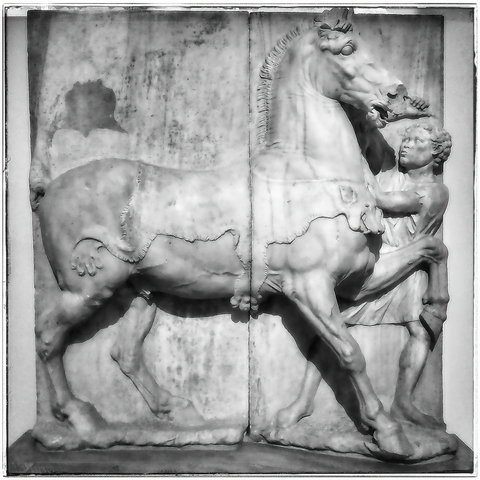
\includegraphics{smallthumb-lesson_I.jpeg}
\setfloatalignment{b}
\end{marginfigure}

\begin{abstract}
\noindent
Queste lezioni si articolano in \textsc{elementi grammaticali}, 
espressi sommariamente, seguiti da \textsc{vocabolari} per il lessico di base 
e da \textsc{frasi da tradurre} dal greco e in greco. 
\
L'approccio è quello del testo-laboratorio di morfosintassi: 
si presenta punto per punto - riprendendone la numerazione - 
l'esposizione di Gleason\cite{gleason1903}.\\
\bigskip
\noindent
Lezione III: qualche nozione generale sul sistema dei nomi del greco antico, la declinazione in O (la seconda declinazione),
vocabolario, esercizi.
\end{abstract}

%\printclassoptions

\newthought{55. Numero.} Ci sono tre numeri: come nei verbi (42)
\sidenote{3 numeri. Dal momento che il duale è raro, le relative flessioni sono riportate nelle sole tavole in appendice.}.

\newthought{56. Genere.} Ci sono tre generi: maschile, femminile e neutro
\sidenote{3 generi. Come in latino.}.

\newthought{57.} Valgono le stesse regole del latino: sono \textit{maschili} i nomi dei maschi; ancora, la maggior parte dei nomi di
\textit{fiumi}, \textit{venti} e \textit{mesi dell'anno}. Sono femminili i nomi delle femmine e della maggior parte dei nomi di 
\textit{nazioni}, \textit{città}, \textit{isole} e \textit{alberi}.
Anche la maggior parte dei nomi che indicano \textit{qualità} o \textit{condizione} sono femminile.  

\newthought{58. Caso.} Il greco antico ha cinque casi: nominativo, genitivo, dativo, accusativo e vocativo
\sidenote{5 casi. Gli usi dell'ablativo latino sono suddivisi tra genitivo e dativo.}.
 
\newthought{59. Declinazione.} Ci sono tre declinazioni dei nomi: la declinazione in \textbf{O} o \textit{Seconda declinazione}, 
la declinazione in \textbf{A} o \textit{Prima declinazione} 
e la declinazione in \textbf{Consonante} o \textit{Terza declinazione}
\sidenote{3 declinazioni.}.

\newthought{60. La declinazione in O.} I temi dei nomi di questa declinazione finiscono in \textbf{ο}, qualche volta allungato in \textbf{ω}.
 
\newthought{61.} I nomi in \textbf{ος} sono di solito maschili, qualche volta femminili; i nomi in \textbf{ον} sono neutri.

\newpage

\newthought{62. Modelli}

\begin{fullwidth}
\begin{table}[!htbp]
  \centering
  \begin{tabular}{l l c l l l l}
    %\toprule
	\multicolumn{7}{c}{\textsc{parole guida}} \\
	\multicolumn{2}{c}{\textbf{δοῦλος,}}              & \textsc{nome latino}    & \textbf{λόγος},               & \multicolumn{3}{c}{\textbf{ὁ σοφός ἄνθρωπος},} \\
	\multicolumn{2}{c}{\textit{schiavo,} \textsc{m.}} & \textsc{corrispondente} & \textit{parola,} \textsc{m.}  & \multicolumn{3}{c}{\textit{l'uomo saggio}} \\
   
	\multicolumn{7}{c}{\textsc{singolare}} \\
    \textsc{n.} & \textbf{δοῦλος} & \textit{servus} & \textbf{λόγος} & \textbf{ὁ}   & \textbf{σοφὸς} & \textbf{ἄνθρωπος}  \\
    \textsc{g.} & \textbf{δούλου} & \textit{servi}  & \textbf{λόγου} & \textbf{τοῦ} & \textbf{σοφοῦ} & \textbf{ἀνθρώπου}  \\
    \textsc{d.} & \textbf{δούλῳ}  & \textit{servo}  & \textbf{λόγῳ}  & \textbf{τῷ}  & \textbf{σοφῷ}  & \textbf{ἀνθρώπῳ}  \\
	\textsc{a.} & \textbf{δοῦλον} & \textit{servum} & \textbf{λόγον} & \textbf{τὸν} & \textbf{σοφὸν} & \textbf{ἄνθρωπον}  \\
	\textsc{v.} & \textbf{δοῦλε}  & \textit{serve}  & \textbf{λόγε}  & \textemdash  & \textbf{σοφὲ}  & \textbf{ἄνθρωπε}  \\
	
	\multicolumn{7}{c}{\textsc{plurale}} \\
	\textsc{n.} & \textbf{δοῦλοι}  & \textit{servi}    & \textbf{λόγοι}  & \textbf{οἱ}   & \textbf{σοφοὶ}  & \textbf{ἄνθρωποι}  \\
    \textsc{g.} & \textbf{δούλων}  & \textit{servorum} & \textbf{λόγων}  & \textbf{τῶν}  & \textbf{σοφῶν}  & \textbf{ἀνθρώπων}  \\
    \textsc{d.} & \textbf{δούλοις} & \textit{servis}   & \textbf{λόγοις} & \textbf{τοὶς} & \textbf{σοφοῖς} & \textbf{ἀνθρώποις}  \\
	\textsc{a.} & \textbf{δούλους} & \textit{servos}   & \textbf{λόγους} & \textbf{τούς} & \textbf{σοφοὺς} & \textbf{ἄνθρωπους}  \\
	\textsc{v.} & \textbf{δοῦλοι}  & \textit{servi}   & \textbf{λόγοι}  & \textemdash   & \textbf{σοφοὶ}  & \textbf{ἄνθρωποι}  \\
    %\bottomrule
  \end{tabular}
  \label{tab:normaltab}
  %\zsavepos{pos:normaltab}
\end{table}
\end{fullwidth}

\newthought{Osservazioni}
\begin{itemize}
\item[\textsc{1.}] Nota le somiglianze tra le terminazioni di \textbf{δοῦλος} e \textit{servus}.  
\item[\textsc{2.}] Osserva come l'articolo determinativo in greco sia declinato, e concordi con il nome a cui si riferisce come un aggettivo. 
Non vi è articolo indeterminativo.
\item[\textsc{3.}] Tieni ben presente le variazioni degli accenti, a partire dal caso nominativo, nelle parola guida declinate sopra.
\end{itemize}



\newthought{63. Vocabolario}

\begin{multicols}{2}

    \noindent \hangindent=1em \textbf{ἄνθρωπος,} \textit{uomo}.  \\
    \noindent \hangindent=1em \textbf{δοῦλος,} \textit{schiavo}.  \\
	\noindent \hangindent=1em \textbf{ἵππος,} \textit{cavallo}.  \\
	\noindent \hangindent=1em \textbf{λίθος,} \textit{pietra}.  \\
	\noindent \hangindent=1em \textbf{λόγος,} \textit{parola, discorso}.  \\
	\noindent \hangindent=1em \textbf{ποταμός,} \textit{fiume}.  \\
	\noindent \hangindent=1em \textbf{υἱός,} \textit{figlio}.  \\
	\noindent \hangindent=1em \textbf{ἀγαθός,} \textit{buono, virtuoso}.  \\
	\noindent \hangindent=1em \textbf{καλός,} \textit{bello}.  \\
	\noindent \hangindent=1em \textbf{σοφός,} \textit{saggio}.  \\
	\noindent \hangindent=1em \textbf{εἰς,} \textit{in} prep. con acc.  \\
	\noindent \hangindent=1em \textbf{ἦν, ἦσαν} \textit{era, erano}.  \\
\end{multicols}

\newthought{64. Leggi e traduci:}
\textsc{1.}~λόγων σοφῶν, ἀνθρώπου ἀγαθοῦ. \quad
\textsc{2.}~ὁ δοῦλος υἱὸν ἔχει σοφόν. \quad
\textsc{3.}~ὁ τοῦ δούλον υἱὸς σοφὸς ἦν. \quad
\textsc{4.}~λόγους δὲ σοφοὺς γράφει. \quad
\textsc{5.}~οὐκ εἰς τόν ποταμὸν ἄγει τοὺσ ἵππους. \quad
\textsc{6.}~παίεις τοὺς τοῦ δούλον υἱούς; \quad
\textsc{7.}~πέμψομεν δὲ τῳ ἀνθρώπῳ ἵππους καλόυς. \quad
\textsc{8.}~ἔχετε, λύομεν, γράφει, θύσουσι, λείψεις, ἁρπάζει.


\hyphenation{sa-cri-fi-che-re-mo}

\newthought{65. Scrivi in greco, con accento e spirito:} 
\textsc{1.}~I figli dello schiavo erano saggi.  \quad
\textsc{2.}~Tirano sassi nel fiume. \quad
\textsc{3.}~Cattura (alcuni) bei cavalli.

\begin{figure*}[!b]
  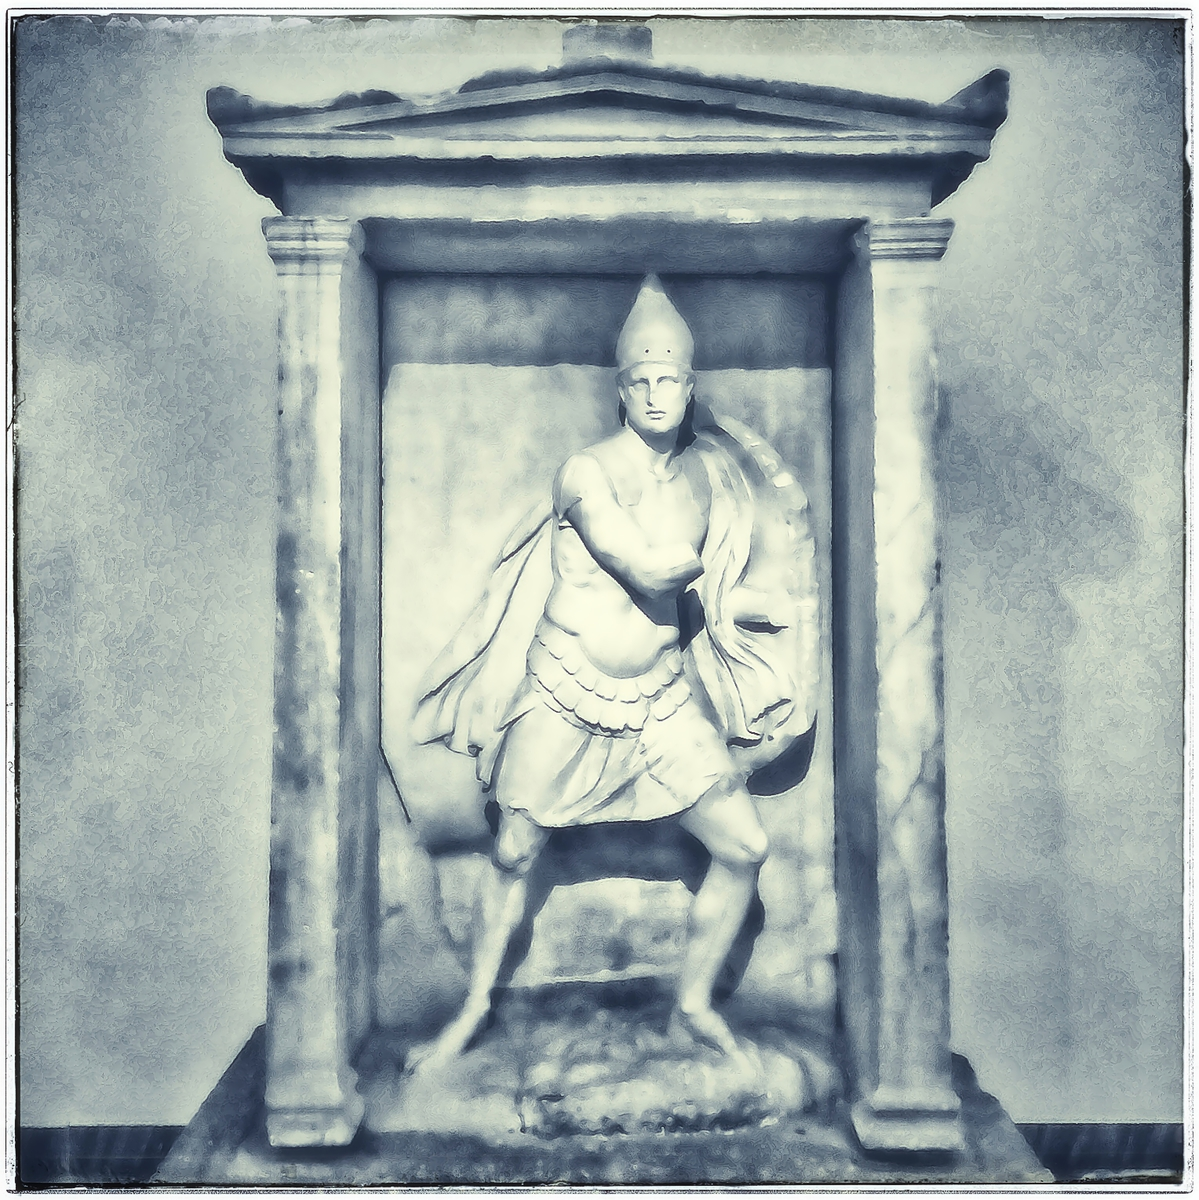
\includegraphics{thumb-lesson_III.jpeg}
  \caption{Museo Nazionale di Archeologia di Atene}
  \label{fig:textfig}
  %\zsavepos{pos:textfig}
  %\setfloatalignment{b}
\end{figure*}

\nobibliography{greekBiblio}
\bibliographystyle{alpha}


\end{document}
